\documentclass[aspectratio=169]{beamer}
\usepackage[utf8]{inputenc}
\usepackage{enumerate,multicol,romannum}
\usepackage{listings}
\usepackage[style=ieee]{biblatex}
\addbibresource{refs.bib}


\usetheme{pug}

\title{Pug}
\subtitle{A custom beamer theme based on metropolis}
\author{Javier Garea}
\institute{University of \LaTeX}
\mydate

% Custom lorem ipsum command. (Due to length)
\newcommand{\lorem}{Lorem ipsum dolor sit amet, consectetur adipiscing elit, sed do eiusmod tempor incididunt ut labore et dolore magna aliqua. Ut enim ad minim veniam, quis nostrud exercitation ullamco laboris nisi ut aliquip ex ea commodo consequat.}


%%%%%%%%%%%%%%%%%%%%%%%%%%%%%%%%%%%%%%%%%%%%%%%%%%%%%%%%
\begin{document}
\titleframe
%%%%%%%%%%%%%%%%%%%%%%%%%%%%%%%%%%%%%%%%%%%%%%%%%%%%%%%%

\section{Introduction}
\begin{frame}{Introduction}
    \lorem
\end{frame}

\section{Lists, columns, pictures, descriptions and tables}
\begin{frame}{Lists}
\begin{multicols}{2}
    Enumerate:
    \begin{enumerate}
        \item Item 1
            \begin{enumerate}
                \item Item 1
            \end{enumerate}
        \item Item 2
            \begin{itemize}
                \item Item 1
            \end{itemize}
        \item Item 3
    \end{enumerate}
    
    Custom bullet enumerate:
    \begin{enumerate}[a)]
        \item Item 1
            \begin{enumerate}[I]
                \item Item 1
            \end{enumerate}
        \item Item 2
            \begin{enumerate}[i]
                \item Item 1
            \end{enumerate}
        \item Item 3
    \end{enumerate}
\end{multicols}

Itemize:
\begin{itemize}
    \item Item 1
        \begin{enumerate}
                \item Item 1
            \end{enumerate}
    \item Item 2
        \begin{itemize}
            \item Item 1
        \end{itemize}
    \item Item 3
\end{itemize}
\end{frame}

\begin{frame}{Columns}
\label{columns}
\begin{columns}
\column{0.5\textwidth}
\lorem
\column{0.5\textwidth}
\lorem
\end{columns}
\end{frame}

\begin{frame}{Pictures}
\label{figures}
\begin{figure}
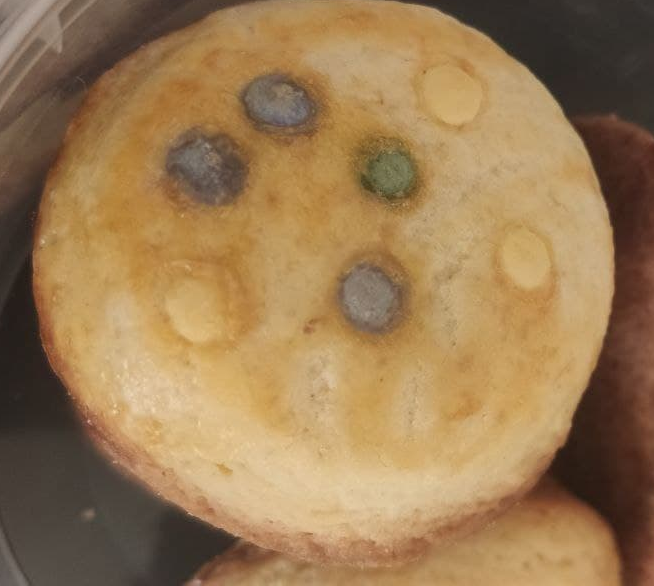
\includegraphics[width=0.3\textwidth]{img/cookie}
\caption{A cookie!}
\end{figure}
\lorem
\end{frame}

\begin{frame}{Descriptions and tables}
    \begin{description}
        \item[API] Application Programming Interface
        \item[LAN] Local Area Network
        \item[ASCII] American Standard Code for Information Interchange
    \end{description}

    \begin{table}
        \begin{tabular}{l | c | c | c | c }
        Competitor Name & Swim & Cycle & Run & Total \\
        \hline \hline
        John T & 13:04 & 24:15 & 18:34 & 55:53 \\ 
        Norman P & 8:00 & 22:45 & 23:02 & 53:47\\
        Alex K & 14:00 & 28:00 & n/a & n/a\\
        Sarah H & 9:22 & 21:10 & 24:03 & 54:35 
        \end{tabular}
        \caption{Triathlon results}
    \end{table}
\end{frame}



\section{Blocks and code}
\newcounter{blocks}
\AtBeginEnvironment{frame}{\addtocounter{blocks}{1}}

\begin{frame}{Blocks \Romannum{\theblocks}}
    \begin{block}{Block}
        \lorem
    \end{block}
    \begin{alertblock}{Alertblock}
        \lorem
    \end{alertblock}
\end{frame}

\begin{frame}{Blocks \Romannum{\theblocks}}
    \begin{definition}
        \lorem
    \end{definition}
    \begin{example}
        \lorem
    \end{example}
\end{frame}

\begin{frame}{Blocks \Romannum{\theblocks}}
    \begin{theorem}[Pythagoras] 
        $ a^2 + b^2 = c^2$
    \end{theorem}
    \begin{corollary}
        $ x + y = y + x  $
    \end{corollary}
    \begin{proof}
        $\omega +\phi = \epsilon$
    \end{proof}
\end{frame}

\begin{frame}[fragile]{Code}
    \begin{lstlisting}[frame=single, caption=Euclidean algorithm, captionpos=b]
function gcd(a, b)
while a ≠ b 
    if a > b
       a := a − b; 
    else
       b := b − a; 
return a;
    \end{lstlisting}
\end{frame}

\section{Standout}

\begin{frame}[standout]{Standout frame}
Standout frame!
\end{frame}


%%%%%%%%%%%%%%%%%%%%%%%%%%%%%%%%%%%%%%%%%%%%%%%%%%%%%%%%
\section{References}

\begin{frame}{References}
   \nocite{*}
   \printbibliography
\end{frame}
%%%%%%%%%%%%%%%%%%%%%%%%%%%%%%%%%%%%%%%%%%%%%%%%%%%%%%%%
\finalframe
\end{document}

